\iffalse
\bibliography{../bib/thesis.bib}
\fi

\chapter{基于标签传播的恶意软件检测算法研究}
恶意软件编程技术的快速发展已经给计算机和网络安全提出了巨大的挑战。因此,反病毒企业与市场急需发展新的有效的方法和框架来保护用户以应对更新的病毒威胁。现有的病毒软件检测技术主要将文件样本作为单一的个体,分析提取文件样本的特征,例如API调用序列、指令序列和二进制字符串等,再运用数据挖掘算法,如朴素贝叶斯、支持向量机等进行病毒检测。文件样本之间的关联关系隐含了大量有价值的信息,忽略他们的关联关系使得分析和检测恶意软件具有一定的局限性。本章从文件样本间关系的角度出发,研究文件样本之间的关联关系和关系类型,提出了基于标签传播的恶意软件检测模型,通过实验验证了标签传播算法在文件关系图上对检测恶意软件的准确性和有效性。
\section{相关研究}


\section{文件关联图的构建}
\subsection{文件关联图类型}
文件关联图根据关联类型以及参与者的不同而不同,
\begin{asparaenum}
\item 文件—文件(File-File)。在文件—文件关联图中,文件与文件之间直接建立关联,若两个文件有共存关系或者有一定的相似度,则就在图中用一条边连接这两个文件对应的节点。
\item 文件—设备(File-Machine)。在文件—设备关联图中,与文件直接相连的是文件所存在的设备(个人电脑、计算机、手机、智能终端等)。通过设备作为过渡点,文件与文件之间建立间接的联系。
\item 文件—聚类(File-Cluster)。在文件—聚类关联图中,通过某种相似度评价算法(例如局部敏感哈希,LSH)将文件在不同维度上进行聚类操作,因此可能会导致同一个文件在不同的维度上会被分到多个聚类中。根据文件与聚类之间的关系,建立文件—聚类关联图。通过聚类作为过渡,文件与文件之间建立间接的联系。
\item 文件—特征(File-Feature)。在文件—特征关联图中,提取文件的特征属性并根据文件属性的紧密程度建立文件与特征间的关系。例如,对于每个Android程序,在AndroidManifest.xml需要声明改程序所需的系统操作权限,将每一种权限作为一个特征即可建立文件与特征之间的关系,即某一权限在程序中被声明则就建立程序与这个特征的联系。
\end{asparaenum}

后三种图均可为二部图,即图中的节点可以分为两部分,一部分为文件,另一部分为另一种实体(即设备、聚类或特征),分属两个部分内的节点互相连接,同一部分内部的节点没有直接连接。本章采用文件—文件关系类型构建文件关联图。
\subsection{图的构建策略}
\label{sec:graphStrategy}
在基于图的半监督学习中,一个良好的图构建方法至关重要。在长期的理论和实践中发现,图的构建方法对最终算法的性能有着重要的影响,甚至在某些情况下构建图的方法比算法更加重要。Maier\cite{maier2008influence}等人研究发现,对于相同的数据以及相同的聚类算法,不同的图构建方法可能会得到不同的结果。Zhu\cite{zhu2005semi}认为能够体现半监督学习假设(半监督平滑性假设、聚类假设和流行假设等)的图才是一个好图。下文列举几种图的构造方法:
\begin{asparaenum}
\item 全连图(Fully connected graphs)。将任意两个节点$v_{i}$和$v_{j}$用一条边连接起来所形成的图称为全连图。相似度较高的两个节点之间的边有较高的权值。全连图的优点是构造方法简单,每条边都被赋予一个权重值(一个可导的权重函数),通过求导的方法即可快速的求解。但是全连图也有明显的缺点,由于任意两个点之间都有边相连,导致了求解过程中庞大的运算量。
\item $k$近邻图($k$-nearest-neighborhood graphs)。若节点$v_{j}$是节点$v_{i}$最近的$k$个近邻之一,则用一条边将这两个节点相连。$k$是控制整个图密度的超参数。$k$近邻图具有良好的自适应性,当样本空间的密度较大时,$k$近邻图的半径就比较小;反之,当密度较小时,图的半径就比较大。在近邻图中,节点$v_{i}$是节点$v_{j}$的$k$近邻并不代表节点$v_{j}$也是节点$v_{i}$的$k$近邻。在构建$k$近邻图时,只要其中一个节点是另一个节点的$k$近邻,则就用一条边连接两个节点,因此在$k$近邻图中每个节点的度(即关联的边数)可能大于$k$。
\item $\epsilon$近邻图($\epsilon$-neighbors graphs)。若节点$v_{i}$和$v_{j}$的距离$d(v_{i},v_{j})\leqslant \epsilon$,则用一条边来连接两个节点。超参数$\epsilon$控制了近邻的半径大小,影响了构造图的连通性。
\item $exp$权重图($exp$-weighted graphs)。上述三种图构造方法主要集中于图的结构构建,没有详细规范图中边权重的计算方法。而$exp$权重图提出了不同的权重计算方法。根据公式$w_{ij}=exp(-d(v_{i},v_{j})^{2}/{\sigma}^{2})$计算连接两个节点的边的权重。超参数$\sigma$影响了权值的衰变。拓展开来,可以为特征的每一维都指定一个超参数$\sigma$。$exp$权重图可以和上述三种构造方法配合使用完成图的构造过程。
\end{asparaenum}

\subsection{构建文件关联图}
\label{sec:fileGraph}
在本章中,我们通过文件样本之间的共存度作为衡量文件样本相似度的标准,以此构建文件样本关联图。定义文件关联图为$G=(V,E,W)$,其中$V$为代表文件样本的节点的集合,$E$为文件样本节点间关系的集合,$e(v_{i},v{j})\in E$,$v_{i}, v_{j}\in V$,表示存在一条边连接节点$v_{i}$和$v_{j}$,$W$为每一条边的权重,即边连接的两个节点的相似度。设$C_{i}$为节点$v_{i}$对应的文件$f_{i}$存在的终端集合。这里我们运用Jaccard相似度来衡量两个文件的共存度,公式如下:
\begin{equation}
sim(f_{i},f_{j})=\frac{\left | C_{i}\cap C_{j} \right |}{\left | C_{i}\cup C_{j} \right |},
\end{equation}
其中,$\left | C \right |$是集合$C$的大小,即文件存在的终端总数。可以看出,共存度的取值是一个介于0和1之间的数。``0''表示两个文件之间没有共存关系,即从未同时存储在同一台终端上; 反之,``1''则表示两个文件之间存在完全的共存关系,可能两个文件存在某种依赖关系。

在实际应用中,文件样本及其存储信息是从实际的用户客户端中采集而来,采集所有的文件样本以及所有的共存信息是不现实、不可行的,因此我们只采集可疑的文件样本以及与已标记文件的共存关系,这就导致了未标记文件样本之间共存关系的丢失。我们使用未标记文件与已标记文件的共存关系来估算未标记文件间的相似度。令$M_{i}$为未标记文件$f_{i}$共存的已标记样本的集合,则未标记文件$f_{i}$和$f_{j}$的相似度为:
\begin{equation}
sim(f_{i},f_{j})=\sum_{m\in M_{i}\cap M_{j}}sim(m,i)*sim(m,j).
\end{equation}

在\ref{sec:graphStrategy}小节,我们讨论了图的构建策略和常用的几种方法。在本章中,我们使用$k$近邻图的构建策略来构建文件关联关系图,若文件样本$f_{i}$是文件$f_{j}$的$k$近邻,则用一条边连接它们,且边的权重为两者的相似度。

为清晰的说明文件关联图构建过程,这里我们选取了一个文件关联的数据集作为例子,如表\ref{tb_dataSample}所示。第一列为文件的ID;第二列为文件的标记,``0''代表当前文件为未标记样本,``1''代表当前文件为良性文件,``-1''代表当前文件为恶意软件;第三列为当前文件样本与恶意软件样本的共存记录;第四列为当前样本与良性文件样本的共存记录;第五列为文件样本存在的终端总数。举例来说,ID为2的文件样本,它是一个存在于两个终端的未标记样本,与ID为4的恶意软件样本共存于一台终端中,与ID为3和ID为6的良性文件样本分别共存于两台终端中。根据所给示例数据,我们选择$k=3$(选择每个节点最近的3个近邻)构建文件关联图,如图\ref{fig:SampleGraph}所示。它是一个无向带权图,图中节点旁标注的数值代表了节点对应的文件样本的编号,同理,每条边上的数值为边的权重,即两节点的相似度。
\begin{table}[!ht]
\caption{文件关联数据库范例}
\label{tb_dataSample}
\centering
\begin{tabular}{ccccc}

\toprule
ID & 标签 & 与恶意软件的共存信息 & 与良性文件的共存信息 & 客户端数量\\
\midrule
1 & 0 & 7(1),8(1),10(1) & 6(1) & 2\\
2 & 0 & 4(1) & 3(2),6(2) & 2\\
3 & 1 & 4(1),8(1) & 5(2),6(3) & 4\\
4 & -1 & 8(1),10(1) & 3(1),6(1) & 2\\
5 & 1 & 8(1) & 3(2),6(1) & 2\\
6 & 1 & 4(1),8(1) & 3(3),5(1) & 4\\
7 & -1 & 10(1) & ------ & 1\\
8 & -1 & 4(1),10(1) & 3(1),5(1),6(1) & 3\\
9 & 0 & ------ & 3(1),5(1),6(1) & 1\\
10 & -1 & 4(1),7(1),8(1) & ------ & 2\\
\bottomrule
\end{tabular}
\end{table}

\begin{figure}[!t]
\centering
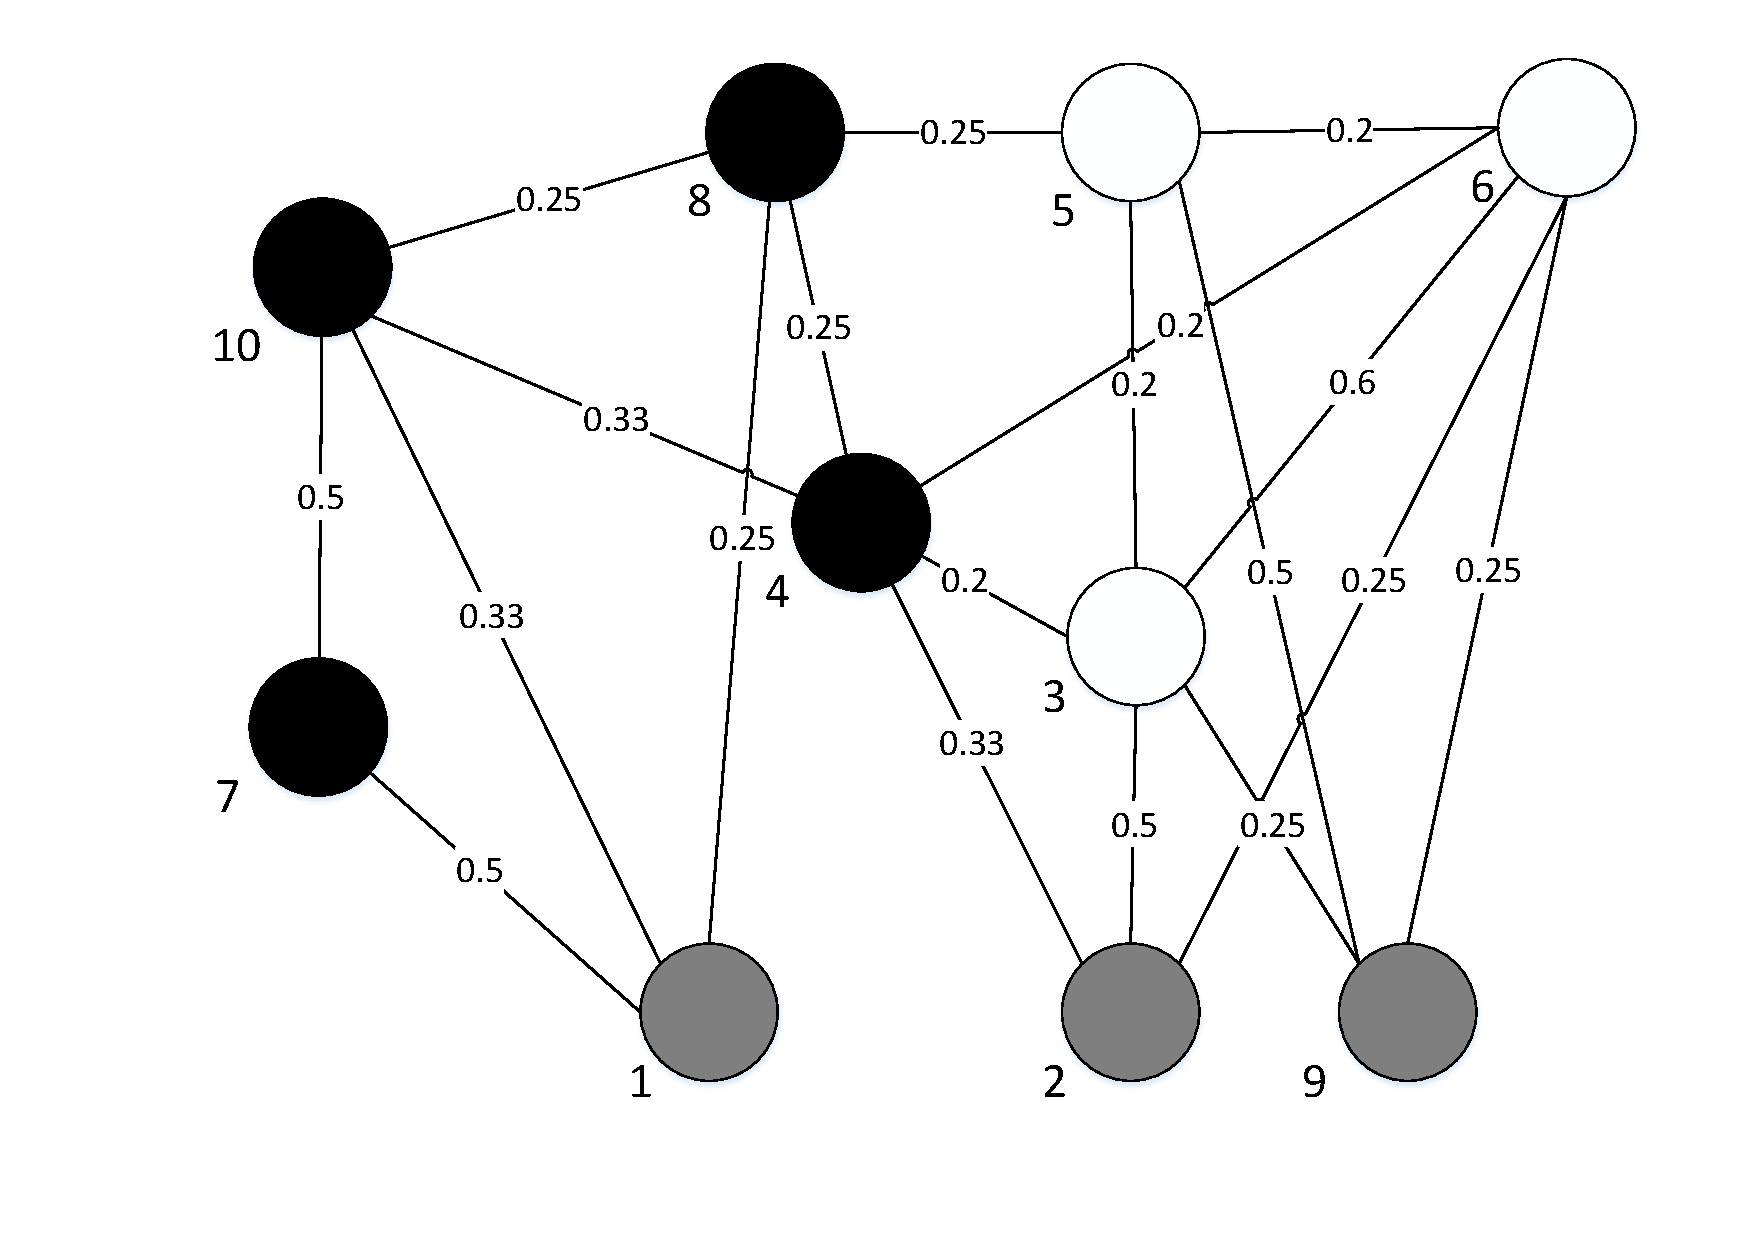
\includegraphics[width=4.5in]{img/chap2/SampleGraph.pdf}
\caption{基于表\ref{tb_dataSample}的文件关联图示例}
\label{fig:SampleGraph}
\end{figure}

\section{标签传播算法}
\label{sec:lp}
数据挖掘算法中,标签数据对于监督学习算法是必需的。然而在很多模式分类的实际应用中,由于样本的标记工作需要昂贵的人力、财力和时间成本,获取大量的标记样本是不实际的。因此,在通常情况下我们面对的是少量的标记样本和大量的未标记样本。如何将未标记样本和标记样本结合起来共同训练模型是近几年研究的热点。

2002年,Zhu等人提出了标签传播算法(LPA,Label Propagation Algorithm)\cite{zhu2002learning},它是一种基于图的半监督学习方法,其基本思想为将已标记节点的标签信息传递给未标记节点以预测未标记节点的标签,高相似度的数据节点倾向于属于同一类别。根据样本间的关系构建关系完全图模型,其中包括已标记节点和未标记节点,节点与节点间的关系则用边来表示,节点间的相似度则表示为边的权重。在标签传递的过程中,已标记节点的标签信息根据节点间的相似度进行传递给邻接节点乃至整个图直至所有的未标记节点达到稳定的标签状态。

标签算法具体如下:设$D_{L}=\left \{ (x_{1},y_{1})...(x_{l},y_{l}) \right \}$为已标记数据,其中$\left \{ y_{1}...y_{l} \right \}$是类别标签。假设类别总数$\left | C \right | $已知,且所有的类别在已标记数据中均存在。令$D_{U}=\left \{ (x_{l+1},y_{l+1})...(x_{l+u},y_{l+u}) \right \}$为未标记数据,$\left \{ y_{l+1}...y_{l+u} \right \}$是不可观测的,通常$l\ll u$(即已标记数据占比很低,未标记数据的数量远大于已标记数据的数量)。该算法的最终目的即为,根据数据集$X$和已知数据标签$\left \{ y_{1}...y_{l} \right \}$来估计$\left \{ y_{l+1}...y_{l+u} \right \}$的取值。

根据数据集中的数据(包括已标记数据和未标记数据)创建一个完全连通图,其中图中每一个节点表示了数据集中的一条数据。节点$i$和$j$之间边的权重用节点间的相似度表示,如下公式:
\begin{equation}
\label{eq:lp_distance}
w_{ij}=\exp\left ( -\frac{d_{ij}^{2}}{{\sigma}^{2}} \right )=\exp\left ( -\frac{{\sum}_{d=1}^{D} {(x_{i}^{d}-x_{j}{d})}^2}{{\sigma}^{2}} \right ),
\end{equation}
其中,$d_{ij}$为两点之间的距离。这里使用欧式距离计算,也可以使用其他的距离计算方法。

定义一个$(l+U)\times C$标签矩阵$Y$,令$Y_{ij}$为节点$x_{i}$被标记为类别$y_{i}$的概率。换言之,矩阵$Y$表示了图中每一个节点的标签概率分布。为衡量节点将标签信息传递给邻接节点的能力,定义概率传递矩阵$T$,
\begin{equation}
\label{eq:lp_transition}
T_{ij}=P(j\rightarrow i)=\frac{w_{ij}}{\sum_{k=1}^{l+u}w_{ij}},
\end{equation}
其中,$T_{ij}$表示从节点$j$跳转到节点$i$的概率,即节点$j$传递标签信息给节点$i$的概率。该算法描述如下:
\begin{asparaenum}
\item 根据公式\ref{eq:lp_distance}计算数据间的相似度以初始化权重矩阵$W$, 并根据矩阵$W$和公式\ref{eq:lp_transition}计算节点$j$到$i$的传播概率,得到标签传递矩阵$T$。
\item 根据已标记数据的标签信息初始化标签矩阵$Y$;若节点$y_{i}$属于类别$C_{j}$,则$Y_{ij}=1$,否则$Y_{ij}$为0。
\item 每个节点将其标签信息传递给邻接节点,其中矩阵$\overline{T}$由矩阵$T$按行归一化得到。
\item 将已标记数据的标签重置为初始值,保证原始的标签信息能够正确传播。重复上一步骤,直至收敛。
\item 根据$y_{i}={\arg \max}_{j}Y_{ij}$,为未标记节点分配标签。
\end{asparaenum}

\begin{algorithm}
\caption{标签传播算法(LPA)}
\label{alg:lp}
\begin{algorithmic}[1]
\Input 未标记数据$D_{U}=(x_{l+1},y_{l+1})...(x_{l+u},y_{l+u})$, 标记数据$D_{L}=(x_{1},y_{1})...(x_{l},y_{l})$及类别集$C$
\Output 未标记数据的类别
\State $initial(D_{U}, D_{L})$ \Comment{初始化相似度矩阵$W$和标签传递矩阵$T$}
\For{$i=0; i<l+u; i++$} \Comment{初始化标签矩阵$Y$}
\For{$j=0; j<\left | C \right | ; j++$}
\State $Y_{ij} = p(y_{i},C_{j})$
\EndFor
\EndFor
\Repeat
\State $Y\leftarrow \overline{T}Y$ \Comment{传播标签信息}
\label{code:lp:propagate}
\State $clamp(D_{L})$ \Comment{限定已标记数据}
\label{code:lp:clamp}
\Until {$Y$ converges}
\State $assignLabel(D_{U})$
\end{algorithmic}
\end{algorithm}

算法\ref{alg:lp}描述了标签传播算法(LPA)的具体步骤。根据已标记数据和未标记数据的排列顺序,划分行规一化矩阵$\overline{T}$为如下4个子矩阵:
\begin{equation}
\overline{T}=\begin{bmatrix}
\overline{T}_{ll} & \overline{T}_{lu} \\ 
\overline{T}_{ul} & \overline{T}_{uu}
\end{bmatrix}
\end{equation}
在算法迭代过程中,由于已标记数据的标签信息始终被限定为原始信息,因此标签矩阵$Y$中前$l$行即子矩阵$Y_{L}$保持不变,算法改变的是未标记数据的部分即子矩阵$Y_{U}$。故算法第\ref{code:lp:propagate}行可改写为
\begin{equation}
Y_{U} \leftarrow \overline{T}_{uu}Y_{U}+\overline{T}_{ul}Y_{L}
\end{equation}
经过有限次迭代后,可以证明该算法收敛至唯一值$Y_{U}=(I-\overline{T}_{uu})^{-1}\overline{T}_{ul}Y_{L}$。

标签传播算法(LPA)只需利用少量的标记数据作为学习导向,利用未标记数据的内部结构和分布规律,即可传播已标记数据的标签信息以及预测未标记数据的标签。该算法操作简单、运算量小,适合大规模数据信息的挖掘和处理。

\section{算法描述}
结合\ref{sec:fileGraph}节构建的文件关联图和\ref{sec:lp}节描述的标签传播算法,我们提出基于标签传播的恶意软件检测算法。在原始的标签传播算法中,根据原始数据点构造了一个完全连通图,在此图的基础上传播节点的标签信息以完成未标记节点的标签学习。本章提出的算法是基于文件样本之间的关联信息的,因此我们单独提出了文件关联关系图的构造策略和算法,以此改进原始标签传播算法中关系图的构造方法。算法\ref{alg:md}阐述了该方法的具体步骤。

\begin{algorithm}
\caption{基于标签传播的恶意软件检测算法}
\label{alg:md}
\begin{algorithmic}[1]
\Input 原始文件列表数据$FileList$
\Output 文件样本的标签
\For{each $f_{i}$ in $FileList$}\Comment{计算每个文件与已知关联文件之间的相似度}
\State $similaityASS(f_{i})$
\EndFor
\For{each $f_{i}$ in $FileList$}\Comment{计算未标记文件样本之间的相似度}
\For{each $f_{j}$ in $FileList$}
\If{$f_{i}$ is unlabled and $f_{j}$ is unlabled}
\State $similaityUnLabel(f_{i},f_{j})$
\EndIf
\EndFor
\EndFor
\State $createGraph(V,E,W,k)$\Comment{构造$k$近邻图}
\State 根据算法\ref{alg:lp}所述的算法进行标签传播
\State 根据标签矩阵标记未标记文件样本的标签
\end{algorithmic}
\end{algorithm}


\section{实验验证}
在本章中,我们提出了一种基于标签传播的恶意软件检测方法,本节将通过两组实验分别来验证算法的可行性和有效性。在第一组实验中,将验证$k$近邻图对于算法准确率的提升并通过实验选择最佳的$k$值;第二组实验将对比本算法与其他基准算法,以验证本算法对恶意软件检测的有效性。

本章中实验的实验环境基于一台普通PC,设备配置为Intel Core i7 2.7G Hz Duo CPU、8GB RAM和500GB硬盘存储,搭建的实验平台为Windows 8操作系统以及JAVA 1.7编程环境。实验过程中使用的性能评价指标如下:
\begin{itemize}
\item \textbf{True Positive(TP)}: 被正确标记为恶意的样本数量。
\item \textbf{True Negative(TN)}: 被正确标记为良性的样本数量。
\item \textbf{False Positive(FP)}: 被错误标记为恶意的样本数量。
\item \textbf{False Negative(FN)}: 被错误标记为良性的样本数量。
\item \textbf{TP Rate(TPR)}: $\frac {TP} {TP+FN}$
\item \textbf{FP Rate(FPR)}: $\frac {FP} {TN+FP}$
\item \textbf{Accuracy(ACC)}: $\frac {TP+TN} {TP+TN+FP+FN}$
\end{itemize}

\subsection{实验数据}
\label{sec:DataDes}
本节介绍实验中所用数据集的相关信息。该数据集由某安全软件企业从真实客户中收集而来,包含69,165个文件样本(其中包括3,095个恶意软件、22,583个良性文件以及43,487个未知文件)以及这些样本之间的关联关系\cite{ye2011combining}。图\ref{fig_Database}为文件关联数据库的结构,包括8个字段:文件ID,文件标签(``1'' 表示当前文件为良性文件, ``-1''表示当前文件为恶意软件,  ``0''代表当前文件为未知文件),文件名,与当前文件共存的恶意软件数量,与当前文件共存的恶意软件ID列表,与当前文件共存的良性文件数量,与当前文件共存的良性文件ID列表,文件存储的客户端数量。

\begin{figure}[!ht]
\centering
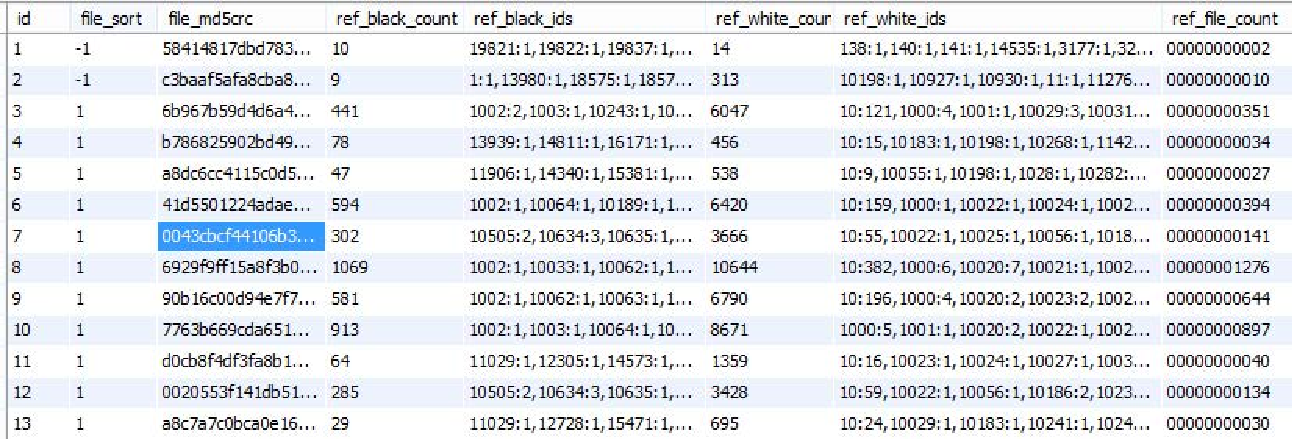
\includegraphics[width=3.5in]{img/chap2/Database.pdf}
\caption{文件关联关系数据库}
\label{fig_Database}
\end{figure}

通过对数据集的分析发现,良性文件的数量远比恶意软件大的多,因此导致了数据分布的不均衡,当然,不仅仅是文件样本数量分布的不均衡,文件之间的关联关系也存在着不均衡分布。图\ref{fig_MalRef}和图\ref{fig_MalRefWht}分别汇总了恶意软件与恶意软件之间的共存关系以及恶意软件与良性文件之间的共存关系。

\begin{figure}[!ht]
\centering
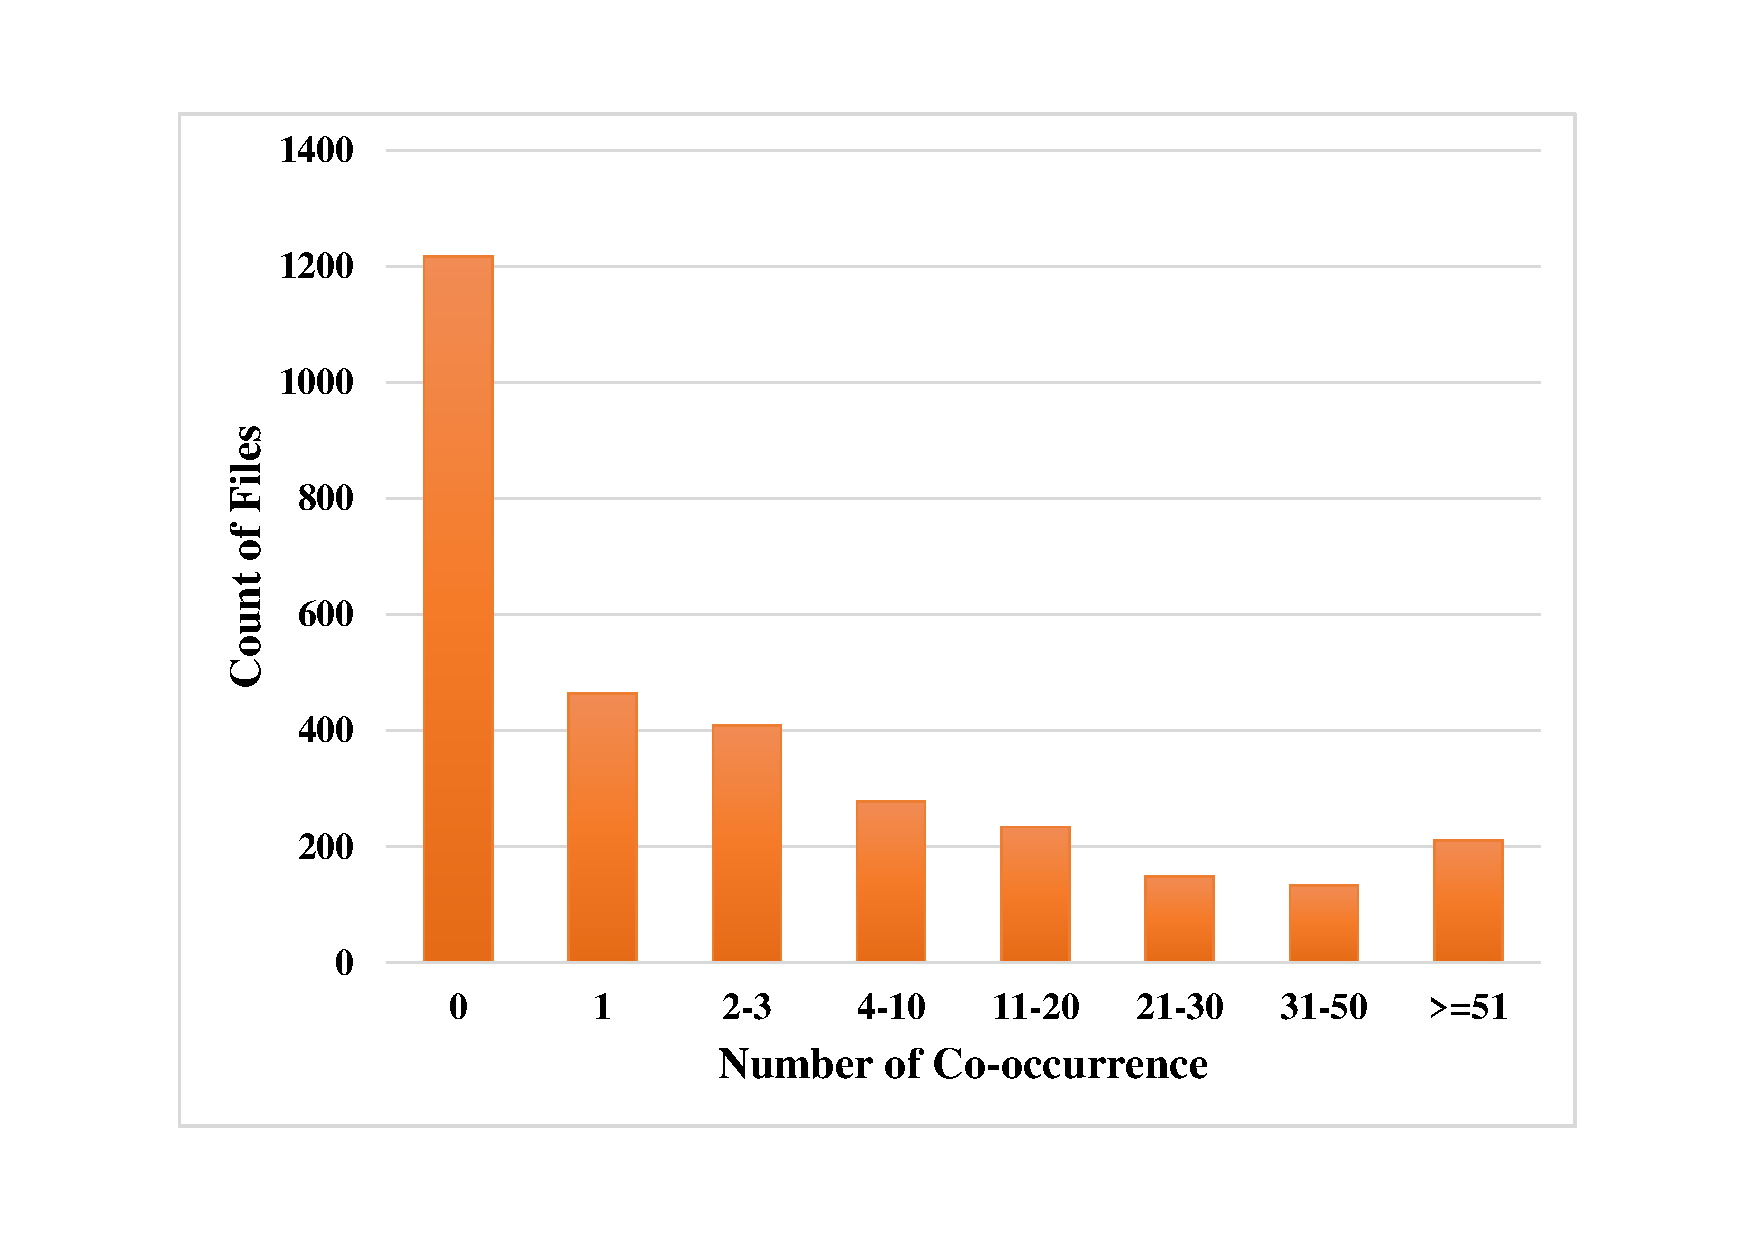
\includegraphics[width=3.5in]{img/chap2/MalRefCount.pdf}
\caption{恶意软件与恶意软件之间的共存关系}
\label{fig_MalRef}
\end{figure}

\begin{figure}[!ht]
\centering
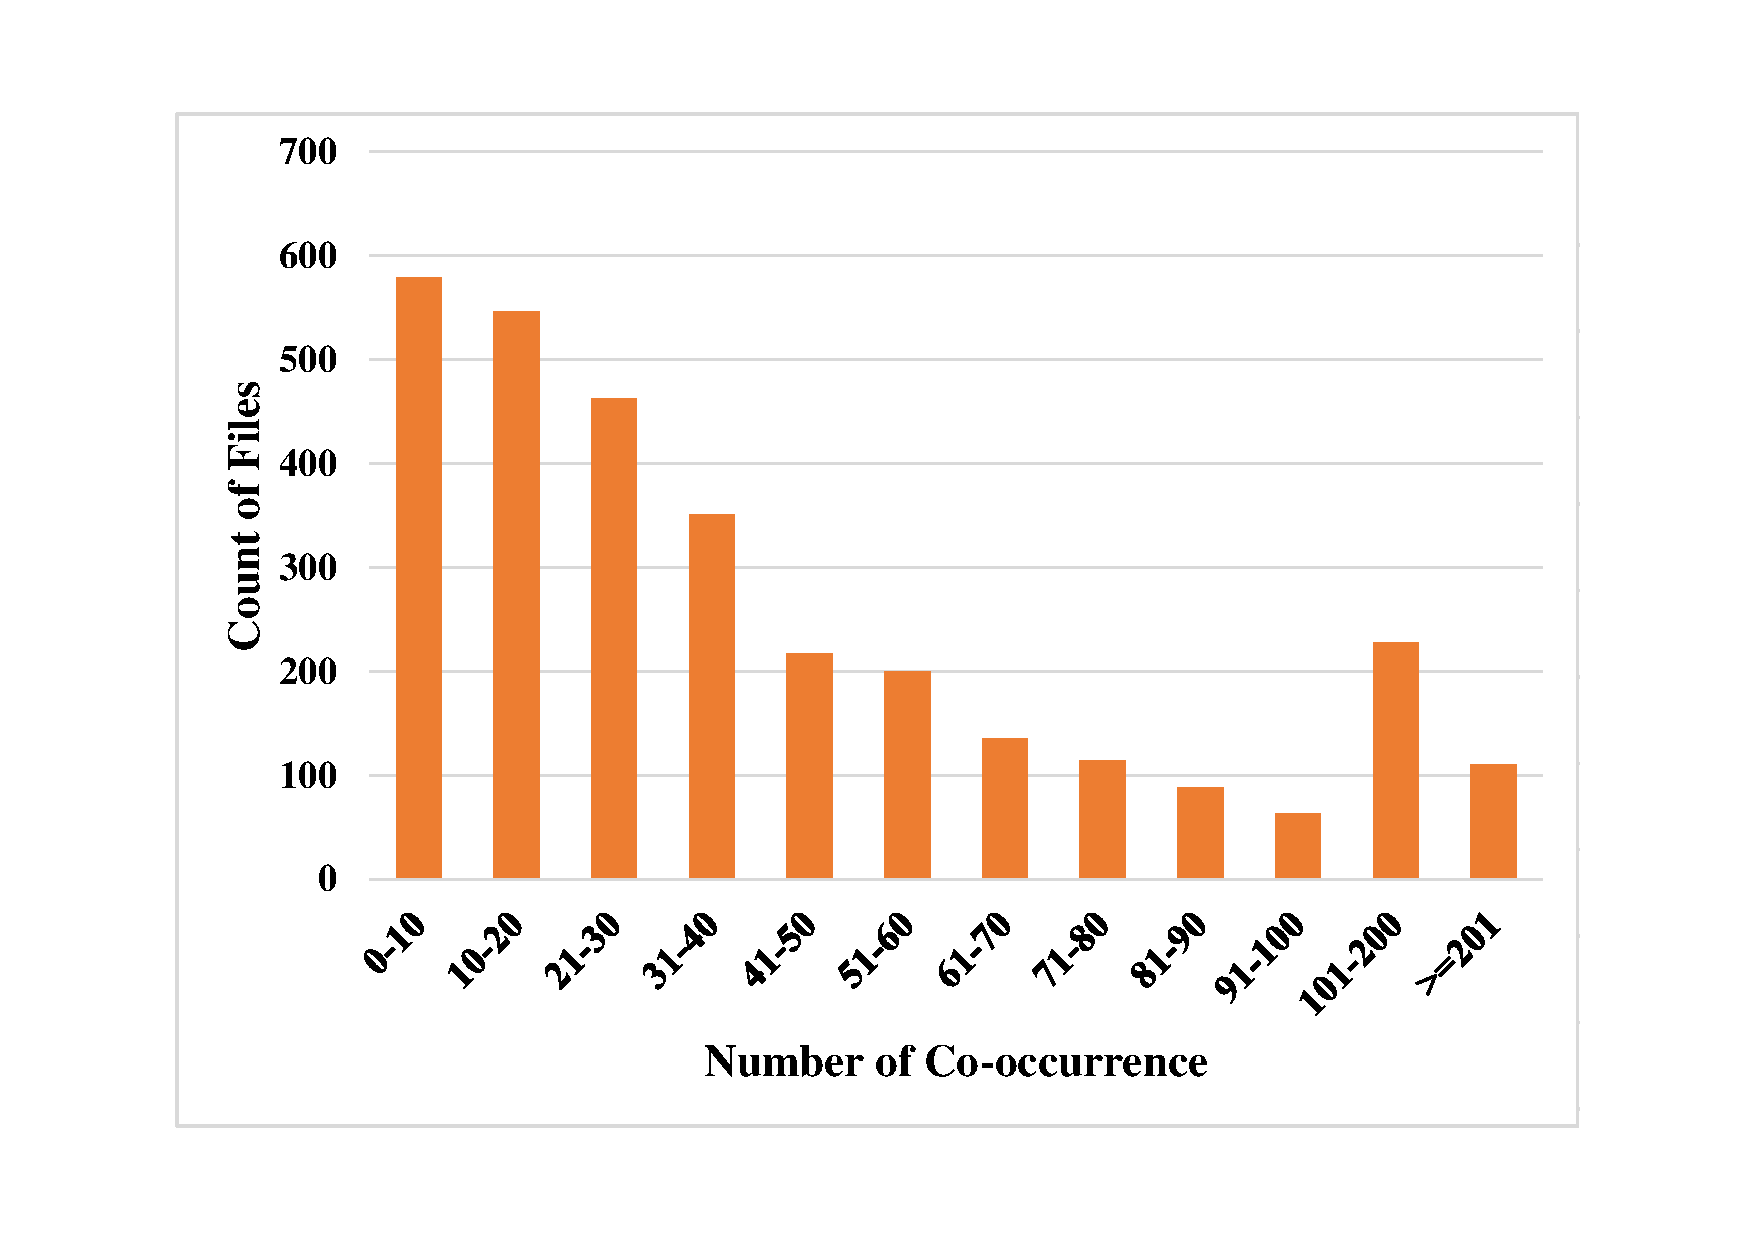
\includegraphics[width=3.5in]{img/chap2/MalRefCountWht.pdf}
\caption{恶意软件与良性文件之间的共存关系}
\label{fig_MalRefWht}
\end{figure}
在本章的实验中,我们从已标记文件样本中随机抽取了3,986个文件(其中包括289个恶意软件,3,697个良性文件)作为测试集,剩余样本作为训练集。

\subsection{$k$NN图构建性能对比分析}
在构建文件关联图时,我们使用了$k$近邻策略过滤数据噪声并选择每个文件样本最相似的邻居样本。本节选择与全连图、$\epsilon$近邻图进行实验对比,验证$k$近邻图的有效性。这里分别选择$\epsilon=0.01$、$\epsilon=0.02$、$\epsilon=0.05$、$\epsilon=0.07$和$\epsilon=0.1$以及$k=10$、$k=30$、$k=50$、$k=70$和$k=100$作为构图参数。通过表\ref{tb_ResKNN}和图\ref{fig_ReskNN}可以看出,运用$k$近邻策略能够明显的提升算法的有效性和准确率。当$k=50$时,对比全连图策略,$k$近邻策略在TP(True Positive)和TN(True Negative)测度上分别能够获得41\%和6.9\%的提高,准确率则可以提升7.96\%。

\begin{table}[!ht]
\renewcommand{\arraystretch}{1.5}
\caption{$k$近邻图性能对比}
\label{tb_ResKNN}
\centering
\begin{tabular}{cccccccc}

\toprule
 & TP & FP & TN & FN & TPR & FPR & ACC\\
\midrule
全连图 & 110 & 301 & 3,396 & 179 & 0.38 & 0.08 & 0.8796 \\
$k=10$ & 109 & 224 & 3,473 & 180 & 0.38 & 0.06 & 0.8986 \\
$k=30$ & 113 & 179 & 3,518 & 176 & 0.39 & 0.05 & 0.9109 \\
$k=50$ & 155 & 67 & 3,630 & 134 & \textbf{0.54} & 0.02 & \textbf{0.9496}\\
$k=70$ & 126 & 139 & 3,558 & 163 & 0.44 & 0.04 & 0.9242 \\
$k=100$ & 122 & 199 & 3,498 & 167 & 0.42 & 0.05 & 0.9082 \\
\bottomrule
\end{tabular}
\end{table}

\begin{figure}[!ht]
\centering
\subfigure[TP VS FN]{
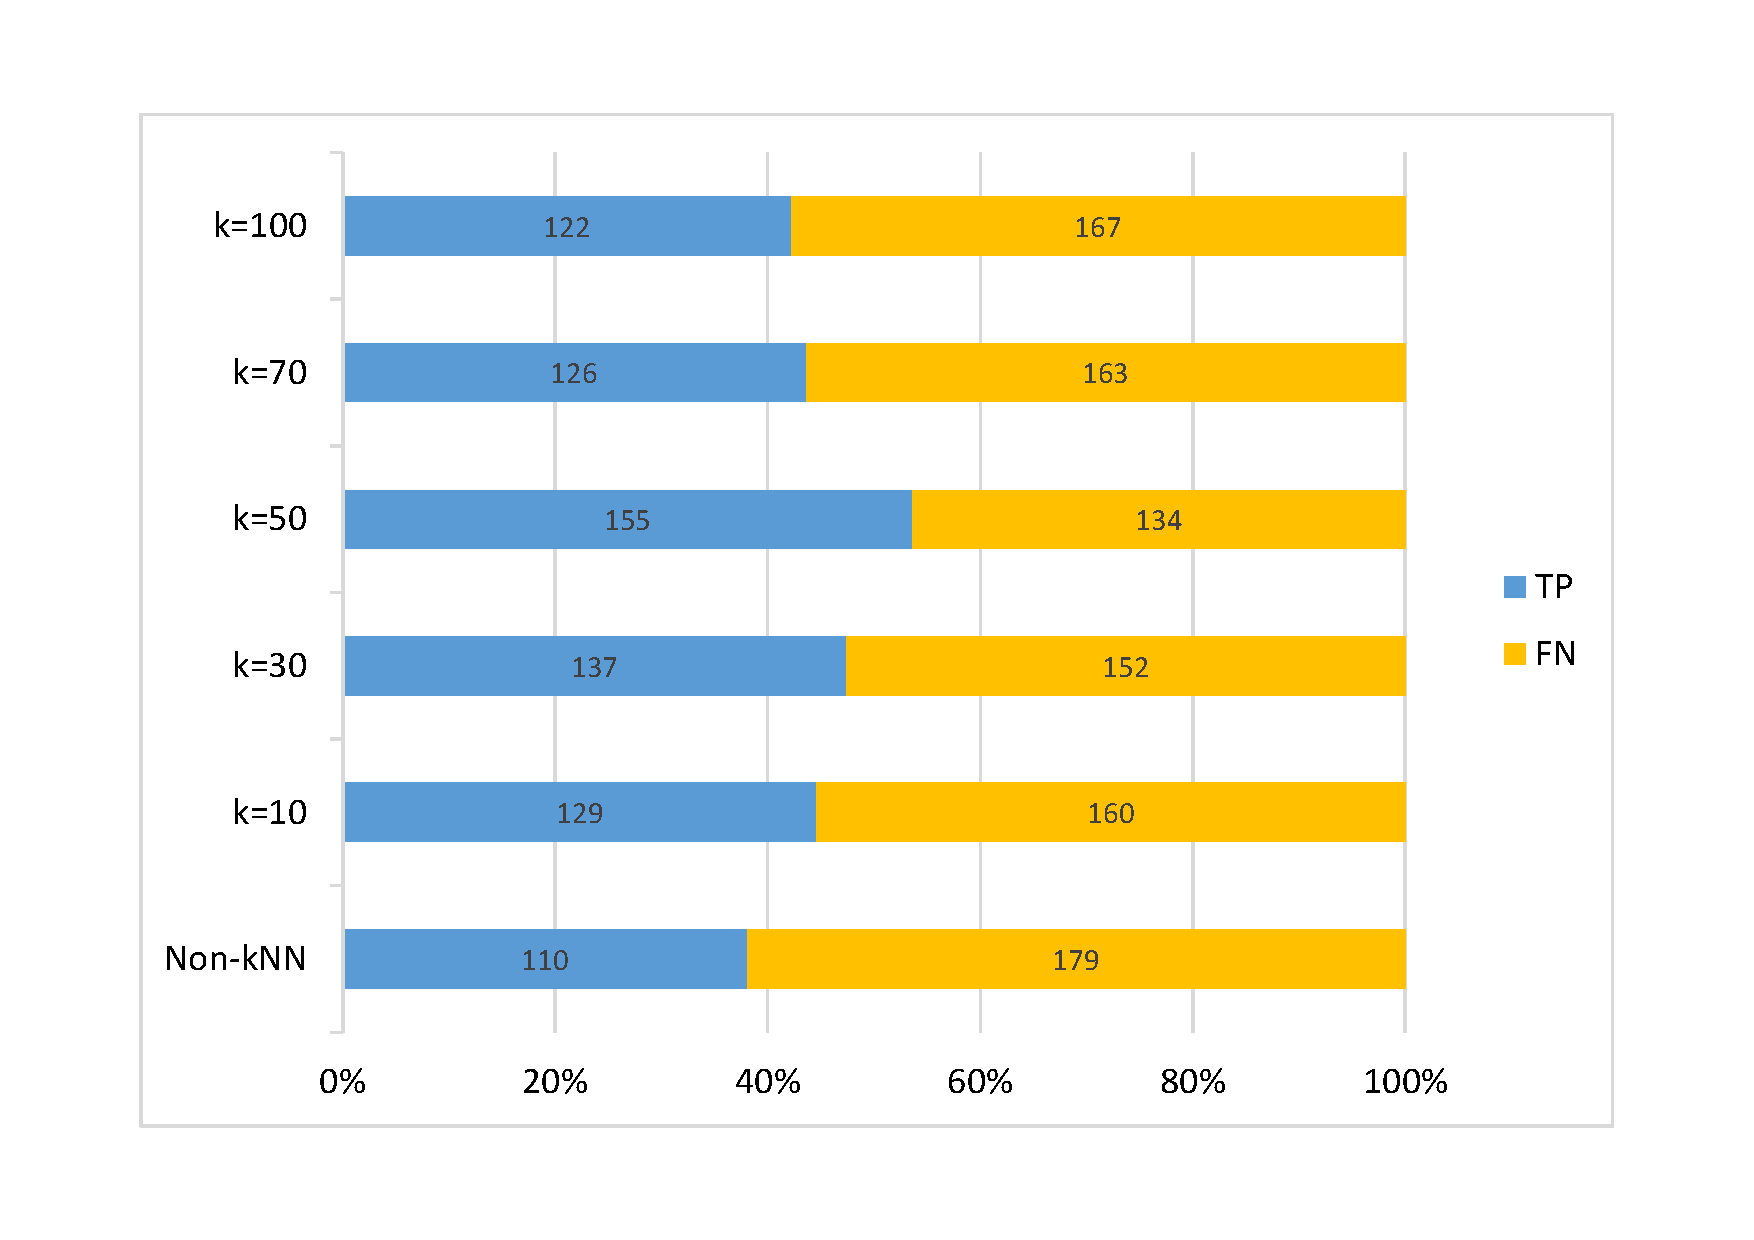
\includegraphics[width=4in]{img/chap2/ResultkNN_TP.pdf}
}
\subfigure[TN VS FP]{
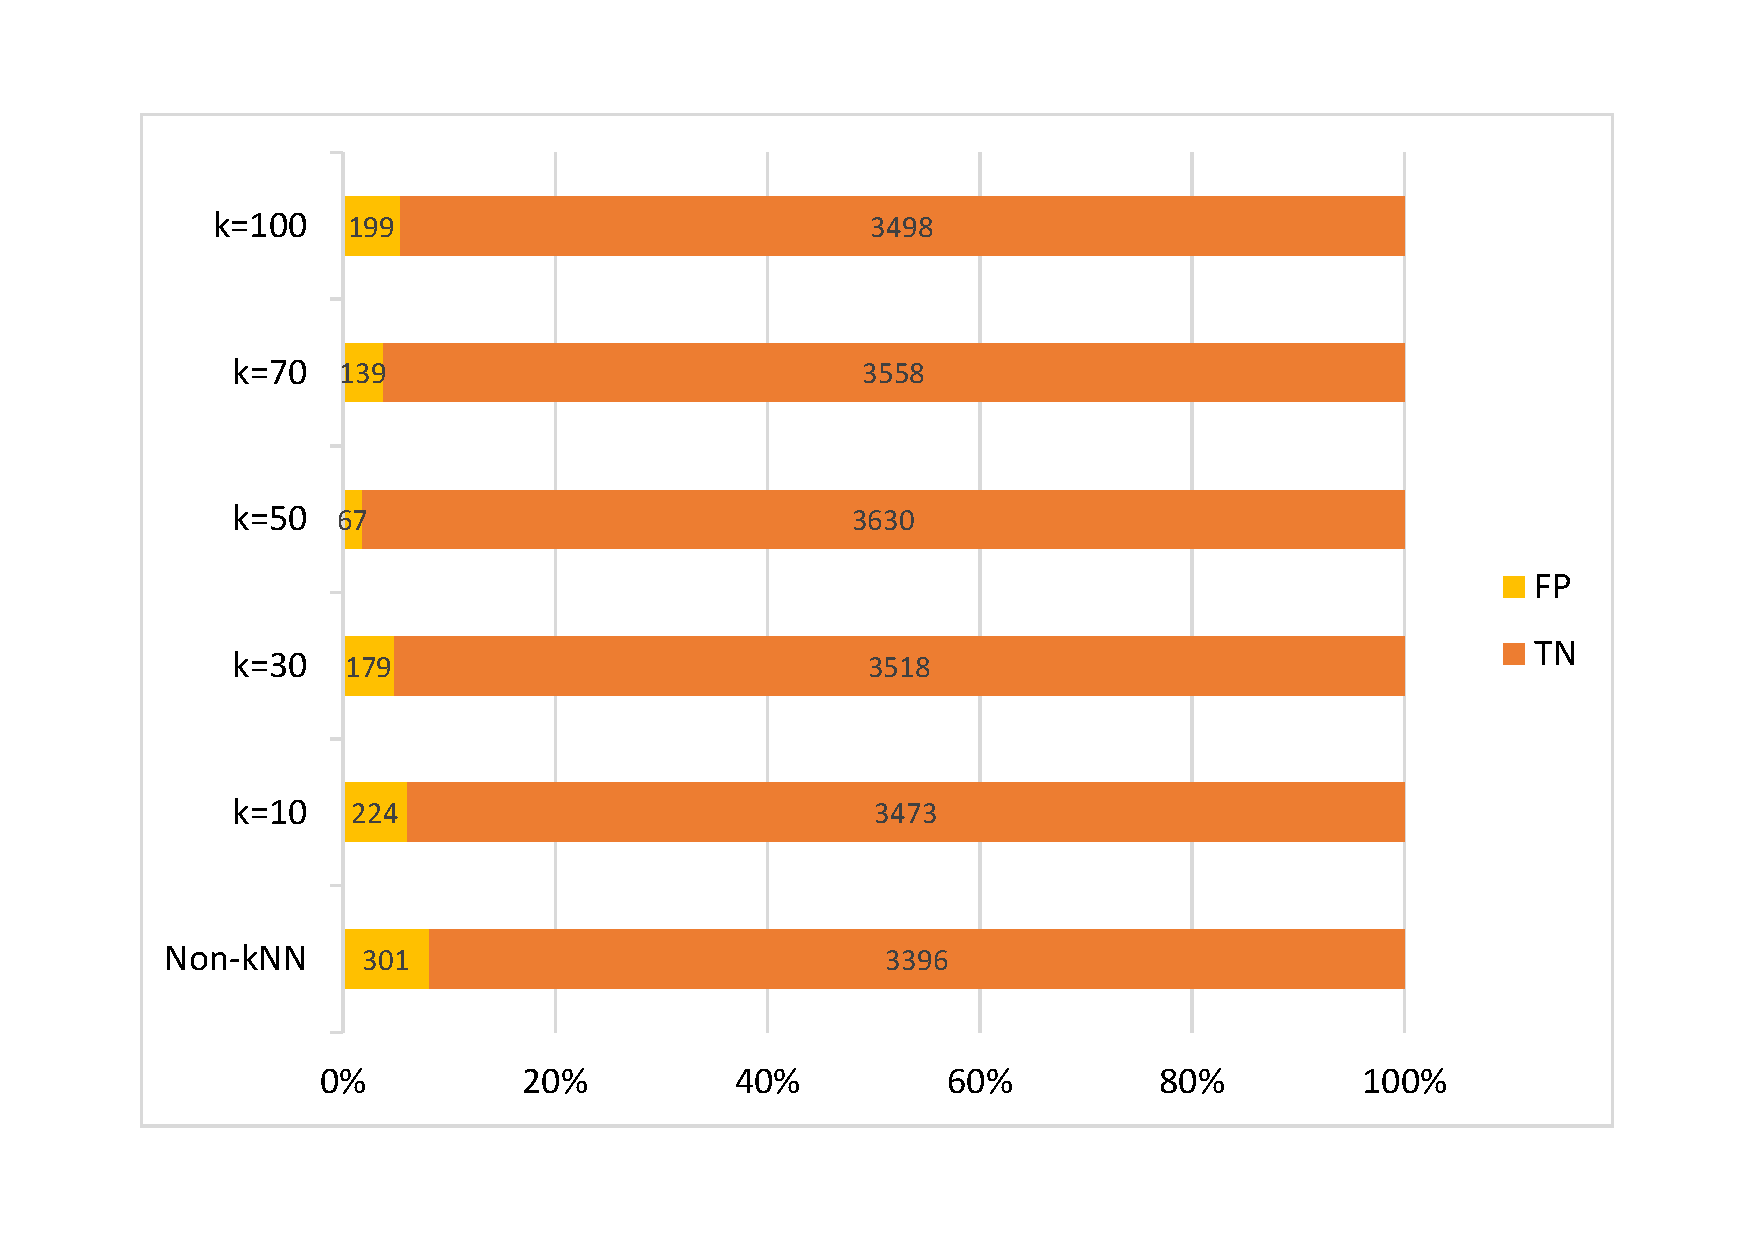
\includegraphics[width=4in]{img/chap2/ResultkNN_TN.pdf}
}
\caption{$k$近邻图性能对比}
\label{fig_ReskNN}
\end{figure}

同时,对比表\ref{tb_ResGraph}和表\ref{tb_ResKNN}的结果,可以看出$k$近邻策略的在每个测度上普遍都优于$\epsilon$近邻图的测度。尤其当$k$取值为50时,算法的准确率明显的高于$\epsilon$近邻图的最优情况。以上实验也验证了$k$取值为50时本算法能够取得最优性能。

\begin{table}[!ht]
\renewcommand{\arraystretch}{1.5}
\caption{三种构图策略对比}
\label{tb_ResGraph}
\centering
\begin{tabular}{cccccccc}
\toprule
 & TP & FP & TN & FN & TPR & FPR & ACC\\
\midrule
全连图 & 110 & 301 & 3,396 & 179 & 0.38 & 0.08 & 0.8796 \\
$\epsilon=0.01$ & 106 & 246 & 3,451 & 183 & 0.37 & 0.8924 \\
$\epsilon=0.02$ & 115 & 213 & 3,484 & 174 & 0.40 & 0.06 & 0.9029 \\
$\epsilon=0.05$ & 121 & 184 & 3,513 & 168 & 0.42 & 0.05 & 0.9117 \\
$\epsilon=0.07$ & 132 & 140 & 3,557 & 157 & 0.46 & 0.04 & 0.9255 \\
$\epsilon=0.1$ & 125 & 174 & 3,523 & 164 & 0.43 & 0.05 & 0.9152\\
$k=50$ & 155 & 67 & 3,630 & 134 & \textbf{0.54} & 0.02 & \textbf{0.9496}\\
\bottomrule
\end{tabular}
\end{table}


\subsection{算法性能分析}
本节将本章提出的恶意软件检测算法与现有的四个恶意软件检测算法进行比较,进一步验证算法的可行性和有效性。四个基准比较算法分别为:AESOP\cite{tamersoy2014guilt}、Malware Distributor Detector(MDD)\cite{venzhega2013graph}、支持向量机(Support Vector Machine, SVM)以及随机森林(Random Forest, RF)。其中,AESOP算法和Malware Distributor Detector算法同样是基于图的算法,因此可以根据文件的关联关系构造算法所需的关联关系图;而支持向量机算法和随机森林算法是基于特征属性的训练算法,因此我们定义每个文件样本的关联属性向量作为训练算法的特征向量:
\begin{equation}
R_{v_{i}}=\left \langle v_{1i},v_{2i},...,v_{ni}\right \rangle
\end{equation}
其中,
\begin{equation}
v_{ji}=\left\{\begin{matrix}
1 & (v_{j},v_{i}) \in E\\ 
0 & \text{其他}
\end{matrix}\right.
\end{equation}
根据上一组实验结果的分析,在构建文件关联关系图时,我们取$k$值为50。

\subsubsection{预测}
从表\ref{tb_ResComparisonWithBaseline}和图\ref{fig_ResComparisonWithBaseline}中可以看出,对比其他几种基准方法,本章提出的基于标签传播的恶意软件检测算法能够有效的发现数据集中的恶意文件样本,在大规模的现实数据中具有较好的表现。

\begin{table}[!ht]
\renewcommand{\arraystretch}{1.5}
\caption{在大规模现实数据上算法的性能对比}
\label{tb_ResComparisonWithBaseline}
\centering
\begin{tabular}{cccccccc}

\toprule
 & TP & FP & TN & FN & TPR & FPR & ACC\\
\midrule
Label Propagation & 155 & 67 & 3,630 & 134 & 0.54 & 0.02 & \textbf{0.9496}\\
AESOP & 198 & 3,385 & 312 & 91 & 0.69 & 0.92 & 0.1279 \\
MDD & 98 & 2,493 & 1,204 & 191 & 0.34 & 0.67 & 0.3266 \\
SVM & 81 & 461 & 3,236 & 208 & 0.28 & 0.12 & 0.8321\\
RF & 69 & 398 & 3,299 & 220 & 0.24 & 0.11 & 0.8449 \\
\bottomrule
\end{tabular}
\end{table}

\begin{figure}[!ht]
\centering
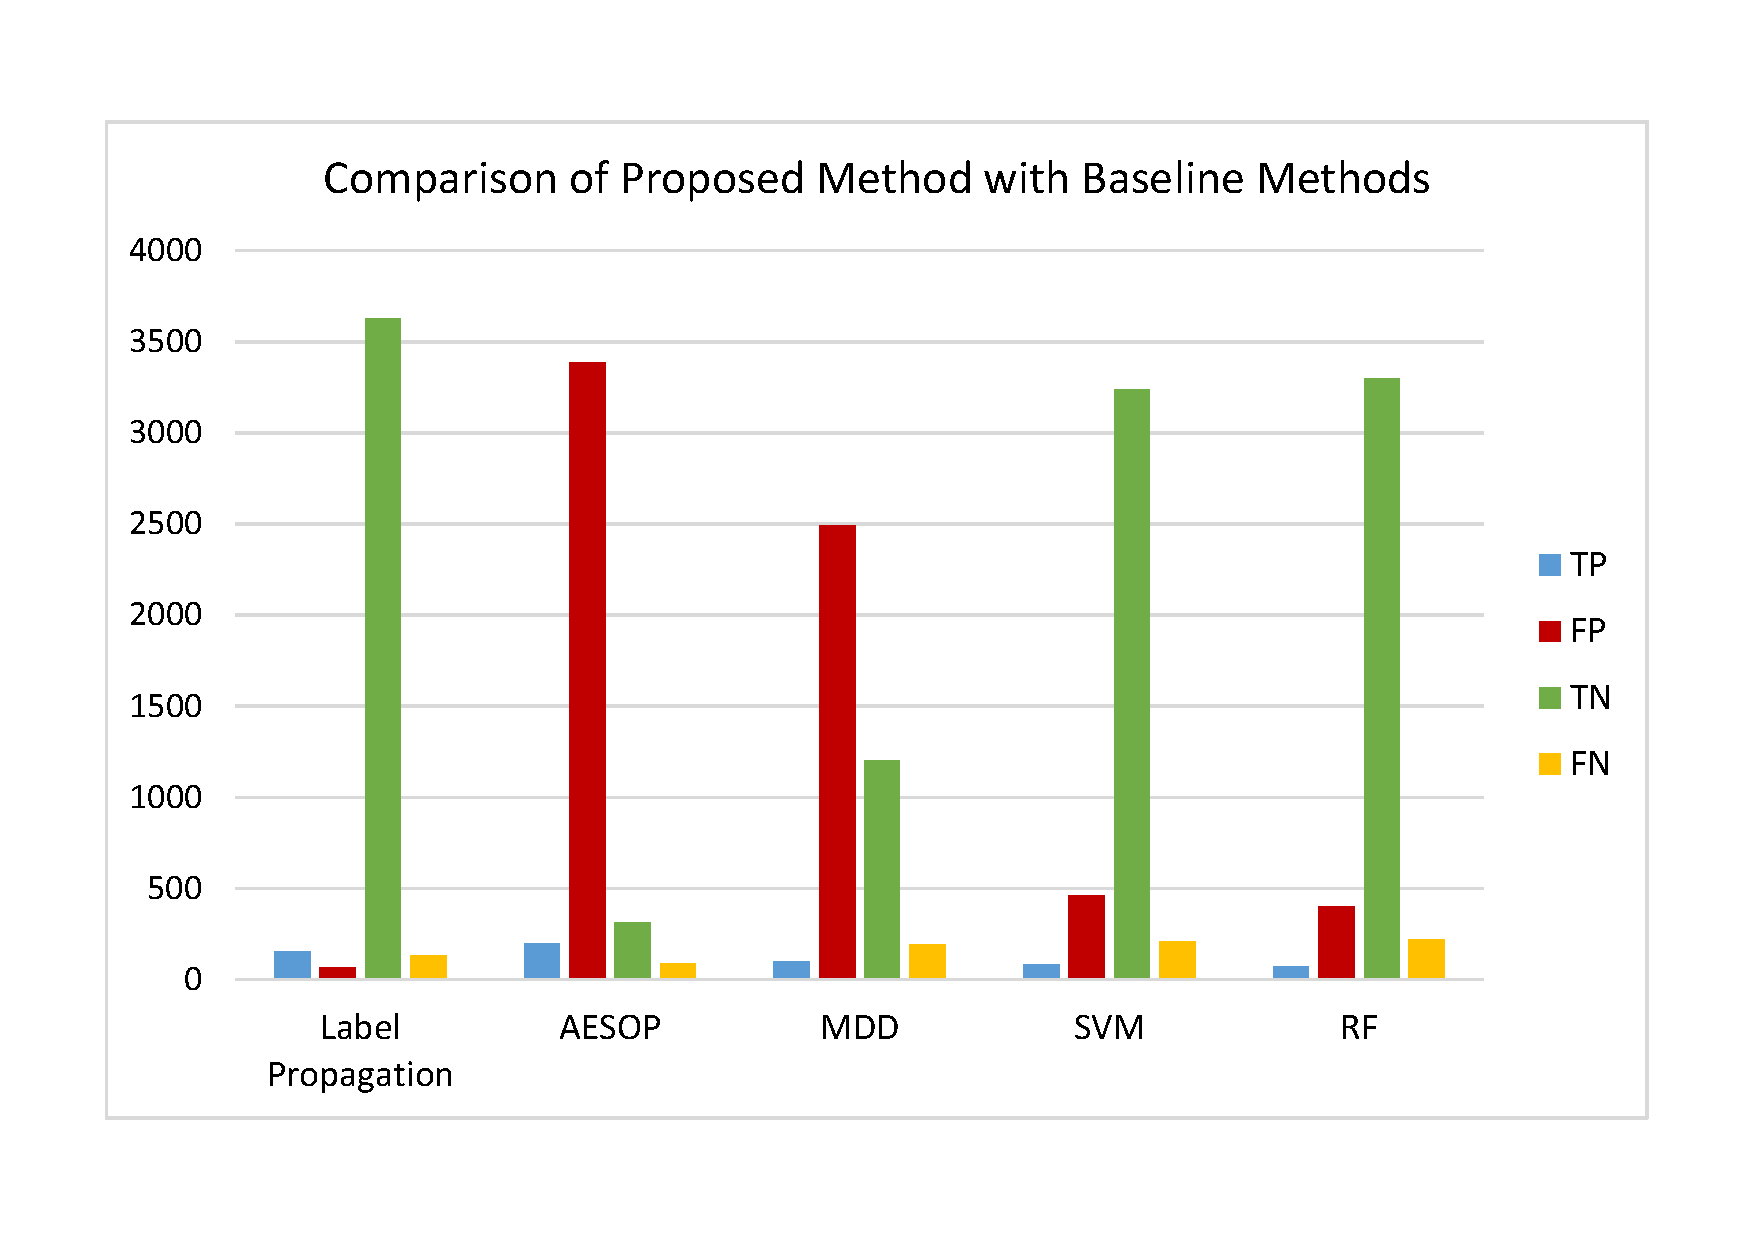
\includegraphics[width=4in]{img/chap2/ResultComparison.pdf}
\caption{在大规模现实数据上算法的性能对比}
\label{fig_ResComparisonWithBaseline}
\end{figure}

\subsubsection{交叉验证}
交叉验证(Cross Validation)是指在某种意义下将原始数据进行分组,一部分做为训练集(Train set),另一部分做为验证集(Test set),首先用训练集对分类器进行训练,再利用测试集来测试训练得到的模型(Model),以此来做为评价分类器的性能指标。通过大量数据集以及不同学习技术进行的大量试验表明10折是获得相对较好误差估计的恰当选择,因此在本实验中使用10折交叉验证(10-fold Cross Validation),将数据集分成十份,轮流将其中的9份作为训练数据,剩余1份作为测试数据,进行试验。每次试验都会得出相应的正确率(或差错率)。10次的结果的正确率(或差错率)的平均值作为对算法精度的估计。在每一次验证中,将测试集的标签设为0(即未标记),标签概率均为0.5(即样本被预测为恶意软件和良性文件的概率是相等的)。基于10折交叉验证的数据结果对比如盒图\ref{fig_Boxplot}所示,图中每个数据盒子中的缺口代表了中位数的95\%置信区间。从图中可以看出,本章提出的基于标签传播的恶意软件检测算法与其他算法相比在检测准确率上能够获得明显的改进和提升。

\begin{figure}[!ht]
\centering
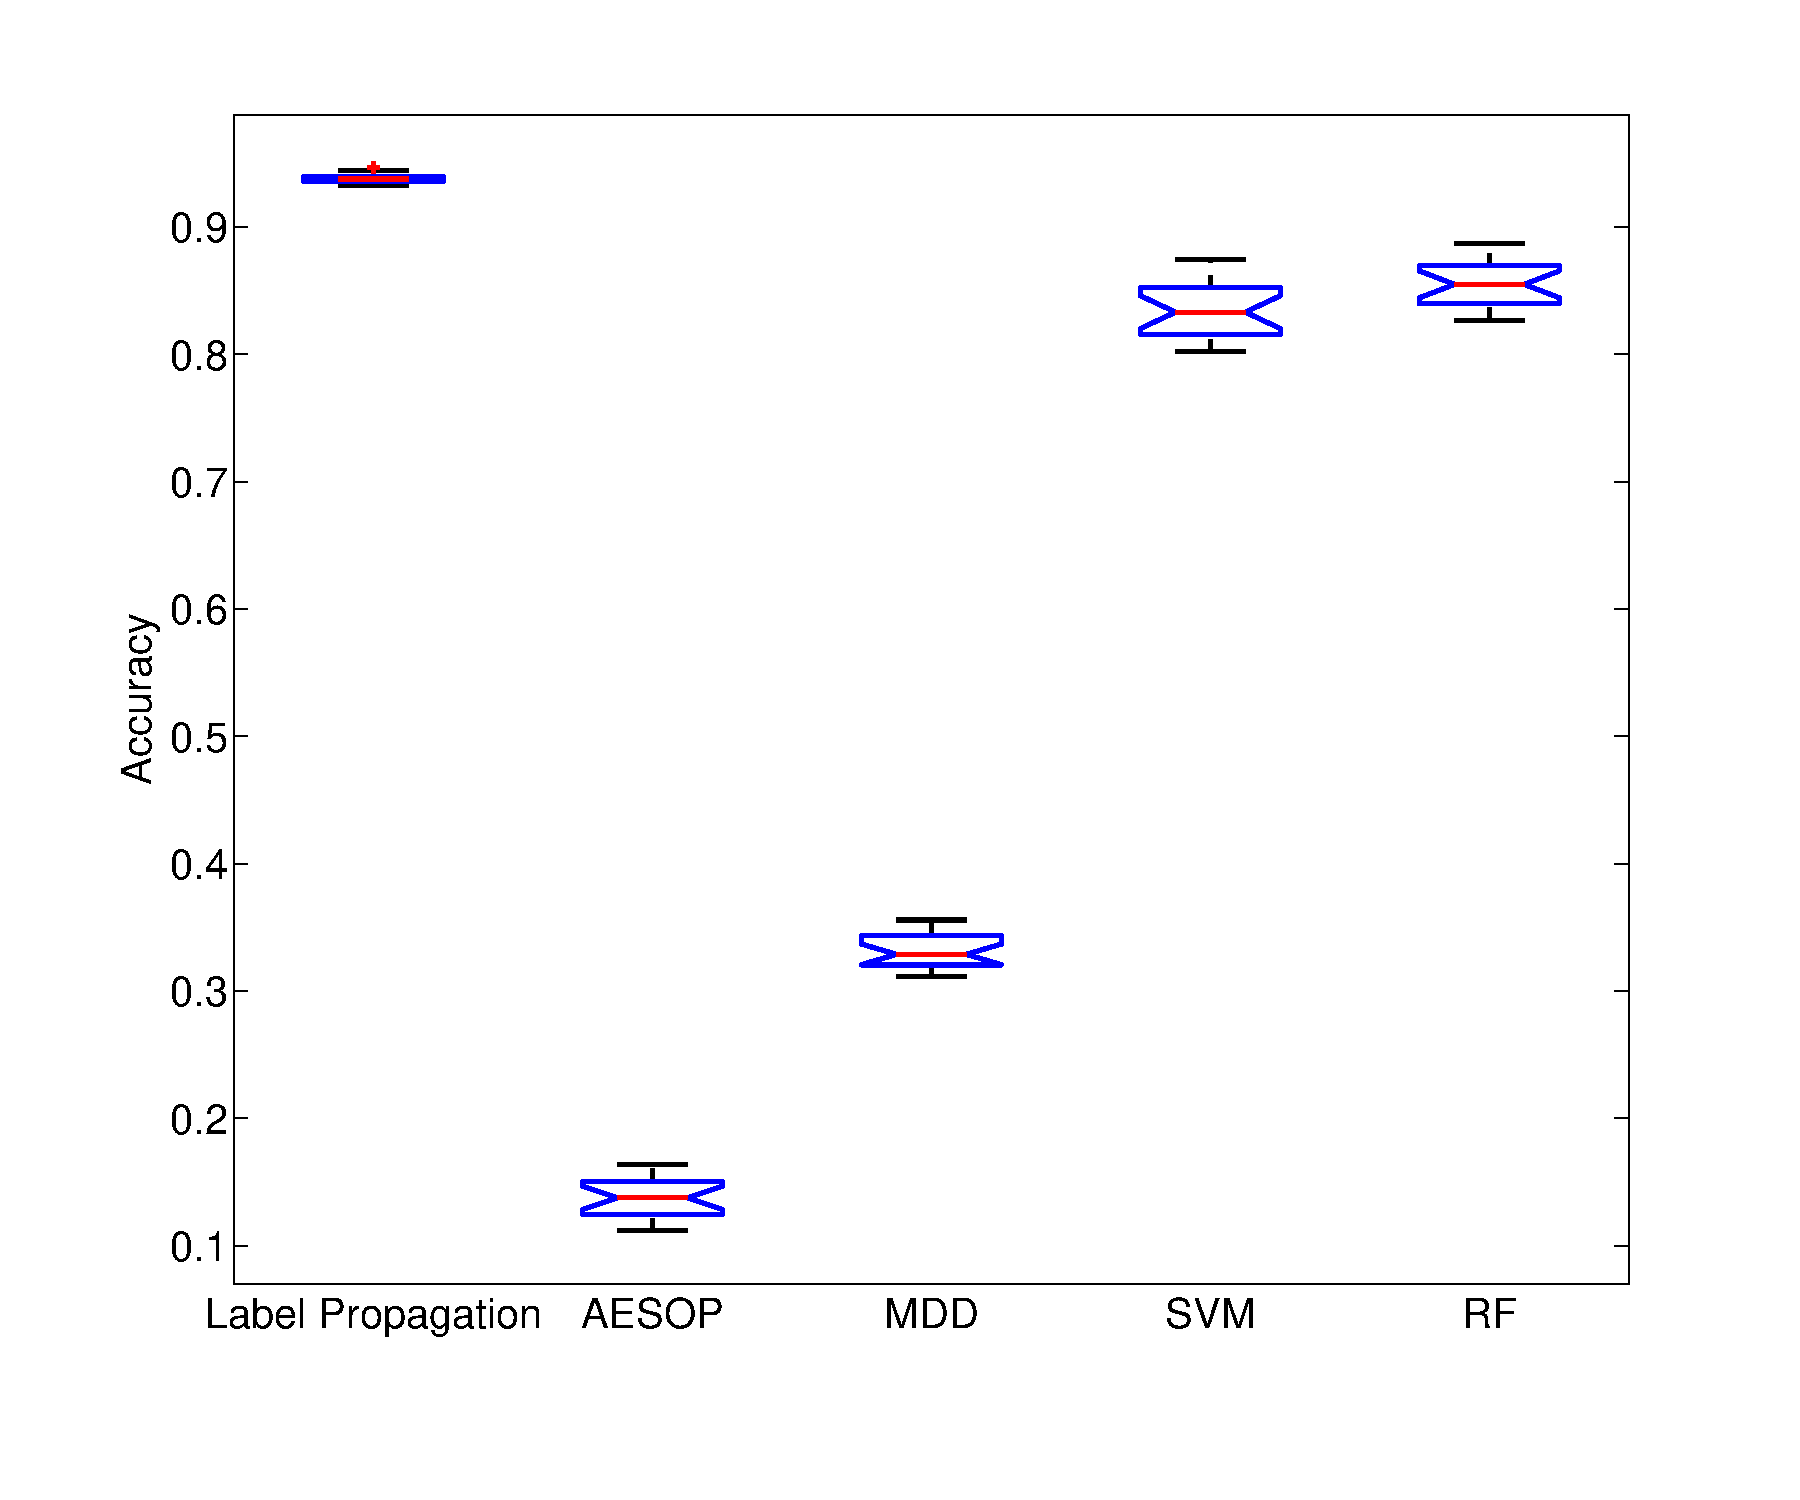
\includegraphics[width=4in]{img/chap2/Boxplot.pdf}
\caption{10折交叉验证准确率对比}
\label{fig_Boxplot}
\end{figure}

\section{本章小结}
本章主要研究了文件样本之间关联关系在恶意软件检测中的相关应用,提出了一种基于标签传播的恶意软件检测方法。采用共存关系作为文件样本之间的关联关系,运用了Jaccard相似度算法来衡量文件样本之间的相似度,在此基础上通过选取每个文件样本的$k$个近邻作为邻接节点来构建文件样本的关联关系图。标签传播算法是一种将已标记节点的标签信息传递给未标记节点的基于图的半监督学习算法。在文件关联图的基础上,利用标签传播算法学习未标记文件样本的标签信息,发现恶意软件样本。将本章中的算法应用于一个从工业界采集得来的大规模真实数据进行实验,通过与真实的数据进行对比,证明提出的算法具有较高的准确性,能够精准的发现新的恶意软件样本。

在后续的研究工作中,需要进一步研究基于图的恶意软件检测算法,分析文件样本的社交关系以及改进基于图的半监督学习算法,提高恶意软件检测的准确率和可靠性。